\chapter{Paralogisms of practical reason}\label{ch:1_chapter}

\epigraphhead[0]{\epigraph{\textit{I loved Ophelia.}\qquad\phantom{}}{--- \textup{Yoda}, \textsc{Star Trek VI}}}


\section{Problematic judgements}\label{sec:first_section}
	
	Internal hyperlinks use the cleveref package (see hyperref\_metadata.tex). Biber is used as backend for the bibliography.
	%
	For more information, see
	%
	the article~\cite{Heidegger:1410}, 
	the arXiv paper~\cite{Schumpeter:2015}, 
	the book~\cite{Nietzsche:2014}, 
	chapter~17 of the book~\cite{Adorno:2014}, 
	the conference~\cite{Schopenhauer:2009}, 
	the proceedings~\cite{Feuerbach:1949}, 
	the url~\cite{Wittgenstein:2015}, 
	the collection~\cite{Popper:2008}, 
	the thesis~\cite{Carnap:2004}, 
	equation~\cref{eq:equation_1},
	\cref{sec:first_section}, 
	\cref{sec:first_section,sec:second_section}, 
	\crefrange{sec:first_section}{sec:1_chapter_MathAnn}, 
	\cref{subsec:1_abc}, 
	\cref{subsubsec:1_def} (all in \cref{ch:1_chapter}),
	\cref{tab:table_page},
	\cref{fig:figure_1}
	the margin note\marginnote{If you use margin notes, enlarge the outer margin to 50--55~mm, and the margin\-parwidth to 30--35~mm (in main.tex).},
	the footnote\footnote{Note that footnote marks come after punctuation marks (see basic\_packages.tex).},
	\href{http://nraontherecord.org/chuck-norris/}{this website},
	and this one: \url{http://xkcd.com/}.
	%
	\begin{theorem}
		\textbf{(Residue Theorem)}
		Let $f$ be analytic in the region $G$ except for the isolated singularities $a_1,a_2,\ldots,a_m$. If $\gamma$ is a closed rectifiable curve in $G$ which does not pass through any of the points $a_k$ and if $\gamma\approx 0$ in $G$ then 
		%
		\begin{equation}
			\paren*{ % determines the size of the braces automatically
			\frac{1}{2\pi i}\int_\gamma f}
			= \sum_{k=1}^m \paren[\Big]{   % enforces \Big braces
					n(\gamma;a_k) \text{Res}
					\paren{f;a_k}  % normal braces
				}	\,.
		\end{equation}
	\end{theorem}
	%
	\mnote{Parentheses with variable size can be set with the \textbackslash{}paren command defined in math\_shortcuts.tex (replaces the \textbackslash{}left and \textbackslash{}right commands). See \href{http://tex.stackexchange.com/questions/7542/for-formal-articles-should-a-displayed-equation-be-followed-by-a-punctuation-to}{this discussion} for information on punctuation before and in mathematical equations.}
	
    \mnote{It's usually considered bad style to both indent paragraphs and add additional space between them. The paragraphing style can be changed in styling.tex (actually, the width of these paragraphs is probably too large to be considered good style anyway). Random text: }\kant[4]
    %
    Margin notes are always\ldots\marginnote{inside the outer margin}. \mnote{Colors are set in basic\_packages.tex and {\color{myRed}hyperref\_metadata.tex}. Deactivate them in the second file for the print version.}
    %
    \ctable[
    	cap = Page dimensions,
    	caption = Page dimensions,
    	label = tab:table_page,
    	pos = h!,
    	]{rll}{
    	\tnote{Vertical lines are rare in professionally typeset books. There's a range of packages for tables: ctables, booktabs, tabularx/y, threeparttable, \ldots}
    	}
	{ \FL  % use \printlength instead of \printlength to get exact values
  	& Width & Height \ML
  	Page & \printlength{\paperwidth} & \printlength{\paperheight} \NN
  	Text & \printlength{\textwidth} & \printlength{\textheight}  \NN
  	Inner \& top margins & \printlength{\dimexpr \oddsidemargin+\hoffset+1in \relax} & \printlength{\dimexpr \headsep+\headheight+\topmargin+\voffset+1in \relax}\NN
  	Outer \& bottom margins & \printlength{\dimexpr \paperwidth-\textwidth-(\oddsidemargin+\hoffset+1in) \relax} & \printlength{\dimexpr \paperheight-\textheight-(\headsep+\headheight+\topmargin+\voffset+1in) \relax}\NN
  	Outer margin (textwidth) & \printlength{\marginparwidth} & - \LL
	} 
    
    \mnote{See the code:}% Here's how you can kill an orphan word at the end of a paragraph (with garamondx and without the following command, there should be a single word at the end of this paragraph)
    \looseness=-1
    \kant[12]
    %

	{\tabcolsep3pt
		\ctable[%	see the documentation of the package
			cap = Lower case letters,
			caption = Lower case letters,
			label = tab:table_lower,
			pos = h!,
			mincapwidth=0em
			]{lllllllllllllllllllllllllll}{
			\tnote{Note the difference between \textit{g}/$g$ and \textit{h}/$h$ for garamondx. \mnote{I used $\mathit{g}$ and $\mathit{h}$ because those were the only versions I could replicate in Illustrator. Attention when using the \textbackslash{}vect command for vectors, it's implemented via bm (see math\_shortcuts.tex).}}
			}{ \FL
			text & a & b & c & d & e & f & g & h & i & j & k & l & m & n & o & p & q & r & s & t & u & v & w & x & y & z \NN
			textbf & \textbf{a} & \textbf{b} & \textbf{c} & \textbf{d} & \textbf{e} & \textbf{f} & \textbf{g} & \textbf{h} & \textbf{i} & \textbf{j} & \textbf{k} & \textbf{l} & \textbf{m} & \textbf{n} & \textbf{o} & \textbf{p} & \textbf{q} & \textbf{r} & \textbf{s} & \textbf{t} & \textbf{u} & \textbf{v} & \textbf{w} & \textbf{x} & \textbf{y} & \textbf{z} \NN
			textsf & \textsf{a} & \textsf{b} & \textsf{c} & \textsf{d} & \textsf{e} & \textsf{f} & \textsf{g} & \textsf{h} & \textsf{i} & \textsf{j} & \textsf{k} & \textsf{l} & \textsf{m} & \textsf{n} & \textsf{o} & \textsf{p} & \textsf{q} & \textsf{r} & \textsf{s} & \textsf{t} & \textsf{u} & \textsf{v} & \textsf{w} & \textsf{x} & \textsf{y} & \textsf{z} \NN
			texttt & \texttt{a} & \texttt{b} & \texttt{c} & \texttt{d} & \texttt{e} & \texttt{f} & \texttt{g} & \texttt{h} & \texttt{i} & \texttt{j} & \texttt{k} & \texttt{l} & \texttt{m} & \texttt{n} & \texttt{o} & \texttt{p} & \texttt{q} & \texttt{r} & \texttt{s} & \texttt{t} & \texttt{u} & \texttt{v} & \texttt{w} & \texttt{x} & \texttt{y} & \texttt{z} \NN
			emph & \emph{a} & \emph{b} & \emph{c} & \emph{d} & \emph{e} & \emph{f} & \emph{g} & \emph{h} & \emph{i} & \emph{j} & \emph{k} & \emph{l} & \emph{m} & \emph{n} & \emph{o} & \emph{p} & \emph{q} & \emph{r} & \emph{s} & \emph{t} & \emph{u} & \emph{v} & \emph{w} & \emph{x} & \emph{y} & \emph{z} \NN
			textsl & \textsl{a} & \textsl{b} & \textsl{c} & \textsl{d} & \textsl{e} & \textsl{f} & \textsl{g} & \textsl{h} & \textsl{i} & \textsl{j} & \textsl{k} & \textsl{l} & \textsl{m} & \textsl{n} & \textsl{o} & \textsl{p} & \textsl{q} & \textsl{r} & \textsl{s} & \textsl{t} & \textsl{u} & \textsl{v} & \textsl{w} & \textsl{x} & \textsl{y} & \textsl{z} \NN
			textit & \textit{a} & \textit{b} & \textit{c} & \textit{d} & \textit{e} & \textit{f} & \textit{g} & \textit{h} & \textit{i} & \textit{j} & \textit{k} & \textit{l} & \textit{m} & \textit{n} & \textit{o} & \textit{p} & \textit{q} & \textit{r} & \textit{s} & \textit{t} & \textit{u} & \textit{v} & \textit{w} & \textit{x} & \textit{y} & \textit{z} \NN
			math & $a$ & $b$ & $c$ & $d$ & $e$ & $f$ & $g$ & $h$ & $i$ & $j$ & $k$ & $l$ & $m$ & $n$ & $o$ & $p$ & $q$ & $r$ & $s$ & $t$ & $u$ & $v$ & $w$ & $x$ & $y$ & $z$ \NN
			bm & $\bm{a}$ & $\bm{b}$ & $\bm{c}$ & $\bm{d}$ & $\bm{e}$ & $\bm{f}$ & $\bm{g}$ & $\bm{h}$ & $\bm{i}$ & $\bm{j}$ & $\bm{k}$ & $\bm{l}$ & $\bm{m}$ & $\bm{n}$ & $\bm{o}$ & $\bm{p}$ & $\bm{q}$ & $\bm{r}$ & $\bm{s}$ & $\bm{t}$ & $\bm{u}$ & $\bm{v}$ & $\bm{w}$ & $\bm{x}$ & $\bm{y}$ & $\bm{z}$ \NN
			bf\&it & \textbf{\textit{a}} & \textbf{\textit{b}} & \textbf{\textit{c}} & \textbf{\textit{d}} & \textbf{\textit{e}} & \textbf{\textit{f}} & \textbf{\textit{g}} & \textbf{\textit{h}} & \textbf{\textit{i}} & \textbf{\textit{j}} & \textbf{\textit{k}} & \textbf{\textit{l}} & \textbf{\textit{m}} & \textbf{\textit{n}} & \textbf{\textit{o}} & \textbf{\textit{p}} & \textbf{\textit{q}} & \textbf{\textit{r}} & \textbf{\textit{s}} & \textbf{\textit{t}} & \textbf{\textit{u}} & \textbf{\textit{v}} & \textbf{\textit{w}} & \textbf{\textit{x}} & \textbf{\textit{y}} & \textbf{\textit{z}}\NN
			textsc & \textsc{a} & \textsc{b} & \textsc{c} & \textsc{d} & \textsc{e} & \textsc{f} & \textsc{g} & \textsc{h} & \textsc{i} & \textsc{j} & \textsc{k} & \textsc{l} & \textsc{m} & \textsc{n} & \textsc{o} & \textsc{p} & \textsc{q} & \textsc{r} & \textsc{s} & \textsc{t} & \textsc{u} & \textsc{v} & \textsc{w} & \textsc{x} & \textsc{y} & \textsc{z}  \LL
		}
	}
	%
	{\tabcolsep2pt
		\ctable[%	
			cap = Upper case letters,
			caption = Upper case letters,
			label = tab:table_upper,
			pos = h!,
			mincapwidth=0em
			]{lllllllllllllllllllllllllll}{}{ \FL
			text & A & B & C & D & E & F & G & H & I & J & K & L & M & N & O & P & Q & R & S & T & U & V & W & X & Y & Z \NN
			textbf & \textbf{A} & \textbf{B} & \textbf{C} & \textbf{D} & \textbf{E} & \textbf{F} & \textbf{G} & \textbf{H} & \textbf{I} & \textbf{J} & \textbf{K} & \textbf{L} & \textbf{M} & \textbf{N} & \textbf{O} & \textbf{P} & \textbf{Q} & \textbf{R} & \textbf{S} & \textbf{T} & \textbf{U} & \textbf{V} & \textbf{W} & \textbf{X} & \textbf{Y} & \textbf{Z} \NN
			textsf & \textsf{A} & \textsf{B} & \textsf{C} & \textsf{D} & \textsf{E} & \textsf{F} & \textsf{G} & \textsf{H} & \textsf{I} & \textsf{J} & \textsf{K} & \textsf{L} & \textsf{M} & \textsf{N} & \textsf{O} & \textsf{P} & \textsf{Q} & \textsf{R} & \textsf{S} & \textsf{T} & \textsf{U} & \textsf{V} & \textsf{W} & \textsf{X} & \textsf{Y} & \textsf{Z} \NN
			texttt & \texttt{A} & \texttt{B} & \texttt{C} & \texttt{D} & \texttt{E} & \texttt{F} & \texttt{G} & \texttt{H} & \texttt{I} & \texttt{J} & \texttt{K} & \texttt{L} & \texttt{M} & \texttt{N} & \texttt{O} & \texttt{P} & \texttt{Q} & \texttt{R} & \texttt{S} & \texttt{T} & \texttt{U} & \texttt{V} & \texttt{W} & \texttt{X} & \texttt{Y} & \texttt{Z} \NN
			emph & \emph{A} & \emph{B} & \emph{C} & \emph{D} & \emph{E} & \emph{F} & \emph{G} & \emph{H} & \emph{I} & \emph{J} & \emph{K} & \emph{L} & \emph{M} & \emph{N} & \emph{O} & \emph{P} & \emph{Q} & \emph{R} & \emph{S} & \emph{T} & \emph{U} & \emph{V} & \emph{W} & \emph{X} & \emph{Y} & \emph{Z} \NN
			textsl & \textsl{A} & \textsl{B} & \textsl{C} & \textsl{D} & \textsl{E} & \textsl{F} & \textsl{G} & \textsl{H} & \textsl{I} & \textsl{J} & \textsl{K} & \textsl{L} & \textsl{M} & \textsl{N} & \textsl{O} & \textsl{P} & \textsl{Q} & \textsl{R} & \textsl{S} & \textsl{T} & \textsl{U} & \textsl{V} & \textsl{W} & \textsl{X} & \textsl{Y} & \textsl{Z} \NN
			textit & \textit{A} & \textit{B} & \textit{C} & \textit{D} & \textit{E} & \textit{F} & \textit{G} & \textit{H} & \textit{I} & \textit{J} & \textit{K} & \textit{L} & \textit{M} & \textit{N} & \textit{O} & \textit{P} & \textit{Q} & \textit{R} & \textit{S} & \textit{T} & \textit{U} & \textit{V} & \textit{W} & \textit{X} & \textit{Y} & \textit{Z} \NN
			math & $A$ & $B$ & $C$ & $D$ & $E$ & $F$ & $G$ & $H$ & $I$ & $J$ & $K$ & $L$ & $M$ & $N$ & $O$ & $P$ & $Q$ & $R$ & $S$ & $T$ & $U$ & $V$ & $W$ & $X$ & $Y$ & $Z$ \NN
			bm & $\bm{A}$ & $\bm{B}$ & $\bm{C}$ & $\bm{D}$ & $\bm{E}$ & $\bm{F}$ & $\bm{G}$ & $\bm{H}$ & $\bm{I}$ & $\bm{J}$ & $\bm{K}$ & $\bm{L}$ & $\bm{M}$ & $\bm{N}$ & $\bm{O}$ & $\bm{P}$ & $\bm{Q}$ & $\bm{R}$ & $\bm{S}$ & $\bm{T}$ & $\bm{U}$ & $\bm{V}$ & $\bm{W}$ & $\bm{X}$ & $\bm{Y}$ & $\bm{Z}$ \NN
			bf\&it & \textbf{\textit{A}} & \textbf{\textit{B}} & \textbf{\textit{C}} & \textbf{\textit{D}} & \textbf{\textit{E}} & \textbf{\textit{F}} & \textbf{\textit{G}} & \textbf{\textit{H}} & \textbf{\textit{I}} & \textbf{\textit{J}} & \textbf{\textit{K}} & \textbf{\textit{L}} & \textbf{\textit{M}} & \textbf{\textit{N}} & \textbf{\textit{O}} & \textbf{\textit{P}} & \textbf{\textit{Q}} & \textbf{\textit{R}} & \textbf{\textit{S}} & \textbf{\textit{T}} & \textbf{\textit{U}} & \textbf{\textit{V}} & \textbf{\textit{W}} & \textbf{\textit{X}} & \textbf{\textit{Y}} & \textbf{\textit{Z}}\NN 
			textsc & \textsc{A} & \textsc{B} & \textsc{C} & \textsc{D} & \textsc{E} & \textsc{F} & \textsc{G} & \textsc{H} & \textsc{I} & \textsc{J} & \textsc{K} & \textsc{L} & \textsc{M} & \textsc{N} & \textsc{O} & \textsc{P} & \textsc{Q} & \textsc{R} & \textsc{S} & \textsc{T} & \textsc{U} & \textsc{V} & \textsc{W} & \textsc{X} & \textsc{Y} & \textsc{Z}  \NN
			m.cal & $\mathcal{A}$ & $\mathcal{B}$ & $\mathcal{C}$ & $\mathcal{D}$ & $\mathcal{E}$ & $\mathcal{F}$ & $\mathcal{G}$ & $\mathcal{H}$ & $\mathcal{I}$ & $\mathcal{J}$ & $\mathcal{K}$ & $\mathcal{L}$ & $\mathcal{M}$ & $\mathcal{N}$ & $\mathcal{O}$ & $\mathcal{P}$ & $\mathcal{Q}$ & $\mathcal{R}$ & $\mathcal{S}$ & $\mathcal{T}$ & $\mathcal{U}$ & $\mathcal{V}$ & $\mathcal{W}$ & $\mathcal{X}$ & $\mathcal{Y}$ & $\mathcal{Z}$ \LL
		}
	}
	%
	{\tabcolsep2.75pt
		\ctable[%
			cap = Greek letters,
			caption = Greek letters,
			label = tab:table_greek,
			pos = h!,
			mincapwidth=0em
			]{llllllllllllllllllllllll}{}{ \FL
			$\mathrm{A}$ & B & $\Gamma$ & $\Delta$ & E & Z & H & $\Theta$ & I & K & $\Lambda$ & M & N & $\Xi$ & O & $\Pi$ & P & $\Sigma$ & T & $\Upsilon$ & $\Phi$ & X & $\Psi$ & $\Omega$  \NN
			$\alpha$ & $\beta$ & $\gamma$ & $\delta$ & $\epsilon$/$\varepsilon$ & $\zeta$ & $\eta$ & $\theta$/$\vartheta$ & $\iota$ & $\kappa$/$\varkappa$ & $\lambda$ & $\mu$ & $\nu$ & $\xi$ & o & $\pi$ & $\rho$/$\varrho$ & $\sigma$/$\varsigma$ & $\tau$ & $\upsilon$ & $\phi$/$\varphi$ & $\chi$ & $\psi$ & $\omega$ \LL
		}
	}	
	%
	{\tabcolsep4pt
		\ctable[%	
			cap = Numbers,
			caption = Numbers,
			label = tab:table_numbers,
			pos = h!,
			mincapwidth=0em
			]{lllllllllllllllllllllllllll}{}{ \FL
			$1$ & $2$ & $3$ & $4$ & $5$ & $6$ & $7$ & $8$ & $9$ \LL
		}
	}	
	%
	\clearpage
	%
	\noindent
	Sets \mnote{see math\_shortcuts.tex}:
	%
	\begin{equation}
		\in \label{eq:equation_1}
			\qquad
		\emptyset 
			\qquad
		\varnothing
			\qquad
		\naturals
			\qquad
		\integers
			\qquad
		\rationals
			\qquad
		\reals
			\qquad
		\complex
			\qquad
		\quaternions
			\qquad
		\octonions
			\qquad
		\lattice
	\end{equation}
	%
	Differential (operators), integrals, sums:
	%
	\begin{equation}
		\partial
		    \qquad
		\diff{x}
		    \qquad
		\delta
		    \qquad
		\eth
		    \qquad
		\laplaceOp
			\qquad
		\discreteLaplaceOp
		  \qquad
		\int_A^B  
			\qquad 
		\oint_\complexPath  
			\qquad 
		\fint_A^B  
			\qquad 
		\sum_{j=0}^{N}  
	\end{equation}
	%
	(In-)equalities, definitions, etc.:
	%
	\begin{equation}
		= 
			\qquad
		\coloneqq  
			\qquad 
		\eqqcolon  
			\qquad 
		\propto
	\end{equation}
	%
	Vectors, matrices:\\\mnote{See the comment on bm for bold italic vectors in math\_shortcuts.tex.}
	%
	\begin{equation}
		\vect{n}   
		  \qquad 
		\unitMatrix
		  \qquad 
		A^\transpose   
	\end{equation}
	%
	Upright exponential, imaginary unit:
	%
	\begin{equation}
		\ee  
			\qquad 
		\ii   
	\end{equation}
	%
	Orthogonal polynomials:
	%
	\begin{equation}
		\hermite
	\end{equation}
	%
	Transformations:
	%
	\begin{equation}
		\legendreTransform
		    \qquad
		\fourierTransform
	\end{equation}
	%
	Miscellaneous:
	%
	\begin{equation}
		\bigO 
			\qquad 
		\binomCoeff{n}{m}
			\qquad
		\hbar 
			\qquad
		\hslash 
			\qquad
		\imath 
			\qquad
		\jmath 
			\qquad
		\ell 
			\qquad
		\wp 
			\qquad
		\infty 
			\qquad
		\backepsilon 
	\end{equation}
	%
	Fock space operators:
	%
	\begin{equation}
	   \cre
	     \qquad
	   \ann
		  \qquad
		\numberOperator
	\end{equation}
	%
	Bras and kets:
	%
	\begin{align}
		&\ketA{n} = \ketA{\vect{n}} =  \braA{n} = \braA{\vect{n}}   
		= \braketA{n}{n} = \braketA{\vect{n}}{\vect{n}}  			\label{eq:equation_3} 
		\qquad\braketBA{n}{n} = \braketBA{\vect{n}}{\vect{n}}  	\\
		&\ketB{n} = \ketB{\vect{n}} =  \braB{n} = \braB{\vect{n}}  		
		= \braketB{n}{n} = \braketB{\vect{n}}{\vect{n}}  		\label{eq:equation_4}
		\qquad\braketAB{n}{n} = \braketAB{\vect{n}}{\vect{n}}  		\\
		&\bigLangle n  = n \bigRangle  = \BigLangle n = n \BigRangle  
		= \bigLLangle n  = n \bigRRangle = \BigLLangle n = n \BigRRangle
			\,.
	\end{align}
	%
	\vfill
	\pagebreak
	%


	\subsection{Physical Reasoning}\label{subsec:1_abc}
		
		\mnote{Random text: }\kant[2]
		%
		\ctable[%	see the documentation of the package
			cap = Short caption for the list of tables,
			caption = The caption above the table,
			label = table_1,
			pos = h
			]{rlcc}{
			\tnote{A footnote.}
			}{ \FL
			& & $\alpha$ & $\beta$ \ML
			&$\gamma$ & $3.1415926535897$ & $932384626433832$ \NN
			&$\delta$ & $79502884197169$ & $399375105820974$ \LL
		}
		%
		\begin{commentDetails}
			Auxiliary explanations, Remove from final text. May stretch over several paragraphs and include equations.
		\end{commentDetails}
		%
		\mnote{Random text: }\kant[3]
		%
		\begin{center}		\vspace{-5mm}
			\begin{equation}			\label{eq:equation_2}
				\begin{tikzpicture}[node distance=7.071mm and 10mm,baseline=(current  bounding  box.center)]
					%
					\coordinate[vertex,label=right:$-\gamma_{\tau,i}$] (tripleVertex);
					\coordinate[left=of tripleVertex] (tripleSink);
					\draw[lineWithArrow] (tripleVertex) -- (tripleSink);
					%
					\coordinate[above right=of tripleVertex,xshift=-2.93mm] (tripleSource1);
					\coordinate[below right=of tripleVertex,xshift=-2.93mm] (tripleSource2);
					\draw[lineWithArrow] (tripleSource1) -- (tripleVertex);
					\draw[lineWithArrow] (tripleSource2) -- (tripleVertex);
					%
					\coordinate[right=of tripleVertex,xshift=3.0mm,label=right:and] (centerCoord);
					%
					\coordinate[vertex,right=of centerCoord,xshift=7.0mm,label=right:$-\gamma_{\tau,i}$] (quadVertex);
					\coordinate[above left=of quadVertex,xshift=2.93mm] (quadSink1);
					\coordinate[below left=of quadVertex,xshift=2.93mm] (quadSink2);
					\draw[lineWithArrow] (quadVertex) -- (quadSink1);
					\draw[lineWithArrow] (quadVertex) -- (quadSink2);
					%
					\coordinate[above right=of quadVertex,xshift=-2.93mm] (quadSource1);
					\coordinate[below right=of quadVertex,xshift=-2.93mm] (quadSource2); %,label=right:$\quad.$
					\draw[lineWithArrow] (quadSource1) -- (quadVertex);
					\draw[lineWithArrow] (quadSource2) -- (quadVertex);
				\end{tikzpicture}
				%
				\hspace{2mm}
				\,.
			\end{equation}
		\end{center}
		%
		\kant[3]
		%
  		\begin{center} 		\vspace{-5mm}
  			\begin{equation}
  				\begin{tikzpicture}[node distance=7.071mm and 10mm,baseline=(current  bounding  box.center)]
  					%
  					\coordinate[vertex] (sink);
  					\coordinate[vertex, right=of sink] (tripleVertex);
  					\draw[lineWithArrow] (tripleVertex) -- (sink);
  					%
  					\coordinate[vertex, right=of tripleVertex,xshift=4.5mm] (quadVertex);
  					\upperloop[linePlain]{quadVertex}{tripleVertex};
  					\lowerloop[linePlain]{quadVertex}{tripleVertex};
  					%
  					\coordinate[above right=of quadVertex,xshift=-2.93mm] (upperSource);
  					\coordinate[below right=of quadVertex,xshift=-2.93mm] (lowerSource); %,label=right:$\quad.$
  					\draw[lineWithArrow] (upperSource) -- (quadVertex);
  					\draw[lineWithArrow] (lowerSource) -- (quadVertex);
  					%
  					% The following lines put Arrowheads on the loops.
  					% Its ugly. But the automatic placement performed an ugly rotation of the arrows.
  					%
  					\coordinate (centerOfUpperLoopTip) at (17.9mm, 7.74mm);
  					\coordinate (centerOfUpperLoopTail) at (17.9mm+0.0001mm, 7.74mm);
  					\draw[black, thick, decoration={markings, mark=at position 1 with {\arrow[scale=1.75]{stealth}}}, postaction={decorate}, draw opacity=0] (centerOfUpperLoopTail) -- (centerOfUpperLoopTip);
  					%
  					\coordinate (centerOfLowerLoopTip) at (18.0mm, -7.74mm);
  					\coordinate (centerOfLowerLoopTail) at (18.0mm+0.0001mm, -7.74mm);
  					\draw[black, thick, decoration={markings, mark=at position 1 with {\arrow[scale=1.75]{stealth}}}, postaction={decorate}, draw opacity=0] (centerOfLowerLoopTail) -- (centerOfLowerLoopTip);
  				\end{tikzpicture}
  				%
  				\hspace{2mm}
  				\,.
  			\end{equation}	
  		\end{center}  
  		%
		\mnote{
		The vertical alignment of inline Feynman diagrams such as 
		%
		\mbox{
			\begin{tikzpicture}[baseline=-0.6ex, node distance=0.6cm]
					\coordinate[vertex] (sink);
					\coordinate[coordinate, right=of sink] (source);
					\draw[lineWithArrowInline] (source) -- (sink);
				\end{tikzpicture}
				,
		}
		can be changed using the ``baseline'' option.}

		\subsubsection{Physical Deduction}\label{subsubsec:1_def}
		
    		\mnote{Random text: }\kant[6]
    		%
			\begin{figure}[tb] 
				\centering
				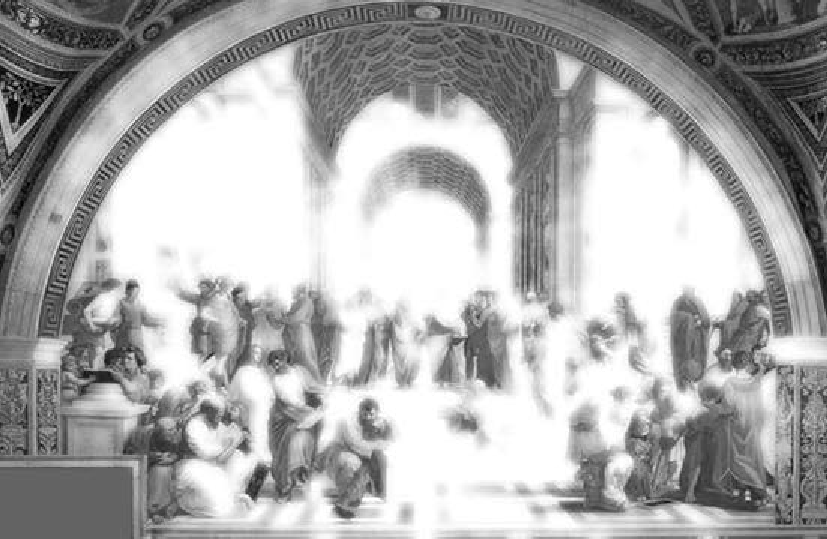
\includegraphics{figure_1}
				\caption[Short caption for the list of figures]{\label{fig:figure_1}
					What we have alone been able to show is that, our understanding depends on the Categories. It remains a mystery why the Ideal stands in need of reason. It must not be supposed that our faculties have lying before them, in the case of the Ideal, the Antinomies.
				}
			\end{figure}    

			\paragraph{Paragraph}\label{par:1_ghi}
				
				\kant[13-15]
				
\section{Paralogisms of practical reason}\label{sec:second_section}

	I used Garamond No.8 for plot labels with sizes of 10~pt or 11~pt. Equations can be reproduced by hand or with the help of LaTeXiT (10~pt chosen here).
	%
	{\footnotesize\begin{equation}
		p(t, n | t_0, n_0) = \braA{n_0}_{t_0} \fint_{(t_0}^{t]} \, \ee^{-\mathcal{S}^\dagger} \, \ketA{n}_{t}  
	\end{equation}}
	%
	\begin{figure}[h!] 
	    \vspace{-7mm}
		\centering
		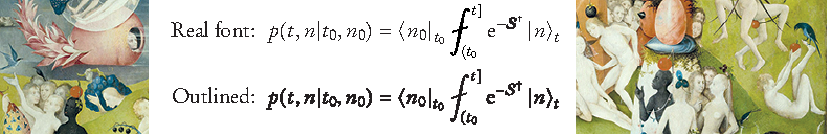
\includegraphics{figure_2}
		\caption[Equations in Illustrator/LaTeXiT]{\label{fig:figure_2}\mnote{Garamond comparison: There's a guide on LaTeXiT in a separate folder. Images exported as ``PDF with outlined font'' look strangely thin (in macOS preview). Good results need some effort.}
		}
	\end{figure}    
    
    \mnote{Random text: }\kant[9]
    
	\cleardoubleemptypage

	\markright{}
	\section[Publication in \textit{Mathematische Annalen}: The ontological manuals]{Publication}\label{sec:1_chapter_MathAnn}

		\begin{center}		
			\vspace*{15mm}
			\onehalfspacing\Large
			\textbf{The ontological manuals}\\
			\doublespacing\normalsize
			\bigskip
			by\\													
			\bigskip		
			\textbf{I. Kant,*\textsuperscript{,1}, M. Heidegger,*\textsuperscript{,1} and F. Nietzsche\textsuperscript{,2}}\\		
			{*equal contribution, \textsuperscript{1}Geiles Department, Geiles Research Center,\\Geile Universit{\"a}t, Super geile Straße 123, 45678 Geile Stadt, Echt geiles Land,\\\textsuperscript{2}Department of Randomness, Random University, Random street 764,\\52464 Random city, random country}\\	
			\bigskip
			\textbf{reprinted on \cpagerefrange{article1Main.1}{article1Main.2}}\\		
			\bigskip			
			with permission from\\
			\textbf{\textit{Math. Ann.}~\textbf{534}(4), 432--458 (1870)},\\
			\textsc{doi:} \href{https://doi.org/10.1007/BF5145949}{10.1007/BF5145949}.\\
			\myCopyrightNormal{} 1870 Springer\\
			% http://www.nature.com/reprints/permission-requests.html	
			\vspace*{\fill}
			Supplemental Material reproduced on \cpagerefrange{article1Supp.1}{article1Supp.2}.
		\end{center}
		
		% WEB: I preferred symmetric margins (e.g. offset=0mm 0mm / scale=1.)
		% PRINT: choose offset and scale to ensure sufficient margins for the binding
		% > approx 2cm inner margin, 1cm outer margin is OK, depends on the journal
		% > further options: trim & clip
		\modifiedincludepdf{pages=-, offset=5mm 0mm, scale=0.94}{article1Main}{manuscripts/article_1} 
		\modifiedincludepdf{pages=-, offset=0mm 0mm, scale=1.}{article1Supp}{manuscripts/supplement_1} 


\begin{subappendices}

	% \renewcommand\thesection{\Alph{section}}%  hides the chapter number
	
	\section{Never-ending regress}\label{sec:1A_abc}
		
		\mnote{The next four pages demonstrate the page layout. The frames are displayed using the ``showframe'' package in temporary.tex.}
		
		\subsection{Necessary principles}\label{subsec:1A_def}

			\kant[13]
		
			\subsubsection{New approaches}\label{subsubsec:1A_ghi}

				\kant[13]
		
				\paragraph{Next steps}\label{par:1A_jkl}

					\looseness=-1
					\kant[2]
					\clearpage
					
					\AddToShipoutPicture*{\ShowFramePicture}
					\kant[36]
					\AddToShipoutPicture*{\ShowFramePicture}
					\kant[37]
					\AddToShipoutPicture*{\ShowFramePicture}
					\kant[38]
					\AddToShipoutPicture*{\ShowFramePicture}
					\kant[39]
					\AddToShipoutPicture*{\ShowFramePicture}
					\kant[40]
					\AddToShipoutPicture*{\ShowFramePicture}
					\kant[41]
					\AddToShipoutPicture*{\ShowFramePicture}
					\kant[42]
					\AddToShipoutPicture*{\ShowFramePicture}
					\kant[43]
					\AddToShipoutPicture*{\ShowFramePicture}
					\kant[44]
					\AddToShipoutPicture*{\ShowFramePicture}
					\kant[45]
					\AddToShipoutPicture*{\ShowFramePicture}
					\kant[46]
					\AddToShipoutPicture*{\ShowFramePicture}
					\kant[13]
			
\end{subappendices}

